% CVPR 2022 Paper Template
% based on the CVPR template provided by Ming-Ming Cheng (https://github.com/MCG-NKU/CVPR_Template)
% modified and extended by Stefan Roth (stefan.roth@NOSPAMtu-darmstadt.de)

\documentclass[10pt,twocolumn,letterpaper]{article}

%%%%%%%%% PAPER TYPE  - PLEASE UPDATE FOR FINAL VERSION
%\usepackage[review]{cvpr}      % To produce the REVIEW version
\usepackage{cvpr}              % To produce the CAMERA-READY version
%$\usepackage[pagenumbers]{cvpr} % To force page numbers, e.g. for an arXiv version

% Include other packages here, before hyperref.


\usepackage{algorithm}
\usepackage{algorithmic}
\usepackage{graphicx}
\usepackage{amsmath}
\usepackage{amssymb}
\usepackage{booktabs}
\usepackage{adjustbox}


% It is strongly recommended to use hyperref, especially for the review version.
% hyperref with option pagebackref eases the reviewers' job.
% Please disable hyperref *only* if you encounter grave issues, e.g. with the
% file validation for the camera-ready version.
%
% If you comment hyperref and then uncomment it, you should delete
% ReviewTempalte.aux before re-running LaTeX.
% (Or just hit 'q' on the first LaTeX run, let it finish, and you
%  should be clear).
\usepackage[pagebackref,breaklinks,colorlinks]{hyperref}


% Support for easy cross-referencing
\usepackage[capitalize]{cleveref}
\crefname{section}{Sec.}{Secs.}
\Crefname{section}{Section}{Sections}
\Crefname{table}{Table}{Tables}
\crefname{table}{Tab.}{Tabs.}


%%%%%%%%% PAPER ID  - PLEASE UPDATE
\def\cvprPaperID{00000} % *** Enter the CVPR Paper ID here
\def\confName{CVPR}
\def\confYear{2023}


\begin{document}
	
	%%%%%%%%% TITLE - PLEASE UPDATE
	\title{Enhancing LiDaR semantic segmentation using model soups }
	
	\author{ Omar Wasfy\\
		{\tt\small omar.wasfy@alexu.edu.eg}
		% For a paper whose authors are all at the same institution,
		% omit the following lines up until the closing ``}''.
	% Additional authors and addresses can be added with ``\and'',
	% just like the second author.
	% To save space, use either the email address or home page, not both
	\and
	Marwan Torki\\
	{\tt\small marwan.torki@alexu.edu.eg}
}
\maketitle

%%%%%%%%% ABSTRACT
\begin{abstract}
	In this paper, we present a pioneering approach for model soups, termed "Iterative Scan Greedy Model Soup," and apply it to the domain of LiDAR semantic segmentation. Leveraging this innovative technique, we augment the state-of-the-art open source code for 2DPASS \cite{yan20222dpass} semantic segmentation and demonstrate its efficacy on both the semanticKitti dataset and the nuscenes dataset. Remarkably, our approach achieves substantial improvements in Mean Intersection Over Union (MIoU) without any increase in prediction time, all while retaining the original model structure.	Our contributions in this work are twofold: Firstly, we successfully extend the application of model soups to LiDAR semantic segmentation, showcasing their adaptability and potential impact on the domain. Secondly, we introduce an optimized and highly efficient version of the existing greedy soup technique, further enhancing the overall performance of the approach. Through comprehensive experiments and rigorous evaluations, our results highlight the significance of the iterative scan greedy model soup in advancing LiDAR semantic segmentation, opening up new possibilities for enhanced perception systems in autonomous driving and related fields.
\end{abstract}

%%%%%%%%% BODY TEXT
\section{Introduction}
\label{sec:intro}

In recent years, semantic segmentation of LiDAR point clouds has emerged as a critical area of research, especially in advancing the scene-understanding capabilities of self-driving cars. The methods for semantic segmentation of LiDAR point clouds can be categorized based on their input modalities into two main groups:

Single Modality LiDAR-Based Input: These methods rely solely on LiDAR data as input. However, due to the sparse nature of LiDAR input, such single-modality-only approaches often face challenges in accurately segmenting complex scenes.

Multiple Modality LiDAR-Based and Camera-Based Input: On the contrary, multiple-modality methods leverage both LiDAR-based and camera-based inputs. By fusing information from both modalities, these techniques attempt to exploit the strengths of each sensor to achieve more robust semantic segmentation.

The open-source model "2D Priors Assisted Semantic Segmentation" (2DPASS)\cite{yan20222dpass} utilizes multiple modalities during the training process to enhance the prediction capabilities of a single-modality model. However, after training, only the single modality (LiDAR) is retained, making it a more practical solution in real-world deployment.

On the other hand, model soups present an efficient approach to improving model performance without modifying the underlying model structure. This technique involves creating an ensemble of models with uniform structures and achieving performance gains akin to traditional ensembling methods without incurring additional prediction costs.

Building upon the foundation of 2DPASS \cite{yan20222dpass}, we propose a novel enhancement to the approach. We introduce a procedure where multiple checkpoints are saved during the training process, and subsequently, a new round of optimization is performed using model soups techniques. By iteratively applying model soups, we aim to further enhance the predictive capabilities of the LiDAR-based single-modality model.

In this paper, we present our iterative scan greedy model soup approach, which leverages the strengths of both 2DPASS \cite{yan20222dpass} and model soups. We demonstrate the effectiveness of our method by conducting extensive experiments on LiDAR semantic segmentation tasks. The results showcase the potential of our approach to achieve notable performance improvements without altering the original model architecture and without incurring additional prediction time.

The contributions of this work are twofold: firstly, the integration of model soups with 2DPASS \cite{yan20222dpass}, which presents a new perspective for enhancing single-modality LiDAR-based semantic segmentation models. Secondly, the validation of our iterative scan greedy model soup approach through empirical evaluations establishes its effectiveness and efficiency in improving semantic segmentation for self-driving cars' scene understanding.




%-------------------------------------------------------------------------
\section{Related Work}
\subsection{ Single-Sensor Methods
}

\subsubsection{Camera-Based Methods:}
Camera-based semantic segmentation aims to predict pixel-wise labels for 2D images, with FCN being a pioneering architecture in this field. Recent advancements have explored multi-scale feature learning, dilated convolution, and attention mechanisms to achieve significant improvements. However, camera-only methods suffer from limitations   in depth sensing and low-light conditions.

\subsubsection{LiDAR-Based Methods:}
LiDAR data is typically represented as point clouds, and various approaches have been developed for processing them. Point-based methods, like PointNet, utilize per-point Multi-Layer Perceptron (MLP) to approximate a permutation-invariant set function. While these methods extract local features from point clouds, they can be inefficient due to time-consuming sampling and grouping algorithms.

\subsubsection{Projection-based methods}
project LiDAR point clouds onto 2D pixels, allowing the use of traditional CNNs. However, such methods suffer from information loss, leading to lower segmentation accuracy.

\subsubsection{Voxel-based frameworks}
, particularly those using SparseConv, have become popular due to their efficiency and effectiveness. These methods store only non-empty voxels in a Hash table and perform convolution operations more efficiently. Recent studies have utilized SparseConv to design powerful network architectures, but they still face challenges in achieving higher segmentation accuracy.

\subsection{Multi-Sensor Methods}

Multi-sensor methods aim to combine information from both cameras and LiDAR, leveraging the strengths of both modalities. Approaches like RGBAL convert RGB images to polar-grid mapping representations and use early and mid-level fusion strategies. PointPainting improves LiDAR network performance by projecting segmentation logits from images into the LiDAR space. PMF explores the collaborative fusion of two modalities in camera coordinates. However, these methods require multi-sensor inputs during both training and inference, making them computationally intensive and less practical for real-world applications.

\subsection{Cross-modal Knowledge Transfer}

Knowledge distillation, initially proposed for model compression, has been extended to transfer knowledge between different models through the alignment of feature representations. Recently, knowledge distillation has been applied to transfer priors across different modalities, using extra 2D images during training to improve inference performance. Various approaches have been explored, such as 2D-assisted pre-training, inflating 2D convolution kernels to 3D, and well-designed teacher-student frameworks.

In this work, we introduce a novel model soup technique applicable to all the above methods. This technique enhances the results without changing the model architecture or incurring extra processing time. By leveraging the complementary information from 2D images, our method improves the segmentation accuracy of LiDAR point clouds in a cross-modal setup. We believe this approach can be a valuable addition to the existing methods for multi-sensor semantic segmentation.
%-------------------------------------------------------------------------

\section{ Approach }


Model souping, alternatively referred to as model averaging, presents an intriguing and innovative paradigm within the realm of ensemble learning strategies. It departs from the customary practice of pooling predictions from discrete models, opting instead for a tactful synthesis of the weights associated with a multitude of individual models. This departure from traditional prediction aggregation highlights model souping's distinctive character, aiming not merely for prediction fusion, but for a nuanced amalgamation of model strengths.

The fundamental tenet of this approach centers around the pursuit of bolstering the overarching performance of the predictive model. By orchestrating a harmonious interplay of diverse model constituents, model souping strives to navigate the intricate balance between bias and variance. This strategic orchestration of model weights empowers the ensemble to harness the unique insights offered by each individual model, thus synergistically augmenting predictive accuracy and promoting robust generalization.

One of the most notable benefits of model souping lies in its inherent ability to counteract the perils of overfitting. By judiciously spreading the influence of different models, the technique inherently introduces a regularization effect that helps mitigate the tendency of the ensemble to tailor itself excessively to the training data. Consequently, the resulting ensemble strikes an equilibrium that deftly sidesteps the pitfalls of overfitting, leading to a more resilient and reliable predictive framework.

In conclusion, model souping stands as a testament to the evolving landscape of ensemble learning paradigms. Its fusion of model weights, carefully curated to accentuate diversity and mitigate overfitting, encapsulates a dynamic approach that aspires to elevate the predictive potential of the ensemble to new heights. This technique serves as a prime example of the ongoing quest within machine learning to push the boundaries of performance by ingeniously orchestrating the synergy between individual model components.






\begin{table}[htbp]
\centering\
	
\small
\begin{tabular}{p{3.5cm} p{4cm}}
		\toprule
		\textbf{Method} & \textbf{Description} \\
		\midrule
		Best ValAcc Model & Choose model with highest validation accuracy ValAcc($\theta_i$) \\
		Ensemble & Combine predictions of models parameterized by $\theta_i$ \\
		Uniform Soup & Average parameter values $\theta_i$ \ \cite{wortsman2022model} \\
		Greedy Soup  & Greedy approach for model ensemble  \cite{wortsman2022model}\\
		Learned Soup & Learn optimized ensemble of models \cite{wortsman2022model} \\
		Pruned Soups & Select subset of models for ensemble \cite{dansereau2023model} \\
		Iterative Uniform Greedy Soup Alg. 1 & Iterative Greedy Soup with uniform weights \\
		Iterative Non-uniform Greedy Soup Alg. 2 & Iterative Greedy Soup with non-uniform weights \\
		\bottomrule
	\end{tabular}
	\caption{Summary of Methods}
\end{table}

\begin{algorithm}[H]
\caption{Iterative Uniform Greedy Soup}
\label{alg:algorithm}
\textbf{Input}: weights of Potential soup ingredients ${\theta_1, ..., \theta_k}$ (optionally sorted in decreasing order of \textbf{ValAcc}($\theta_i$))\\
\textbf{Parameter}:epochs\\
\begin{algorithmic}[1] %[1] enables line numbers
\STATE soupList = emptyList
\STATE bestValAcc = 0
\FOR{epoch=1 to epochs}
\FOR{i=1 to k}
\STATE potentialSoupList $\leftarrow$ AddToSoupList($\theta_i$)
\IF {\textbf{ValAcc}(potentialSoupList) $>=$ bestValAcc}
\STATE bestValAcc = \textbf{ValAcc}(potentialSoupList)
\STATE soupList $\leftarrow$ potentialSoupList
\ENDIF
\ENDFOR
\ENDFOR
\STATE \textbf{return} weights of the final soup $\theta_{soupList}$
\end{algorithmic}
\end{algorithm}



\begin{algorithm}[H]
\caption{Iterative Non Uniform Greedy Soup}
\label{alg:algorithm}
\textbf{Input}: weights of Potential soup ingredients ${\theta_1, ..., \theta_k}$ (optionally sorted in decreasing order of \textbf{ValAcc}($\theta_i$))\\
\textbf{Parameter}:epochs,weightSearchCount,countUniqueCheckpointsEnable,
cummulativeWeightEnable
\begin{algorithmic}[1] %[1] enables line numbers
\STATE soupList = emptyList
\STATE bestValAcc = 0
\FOR{pass=1 to N}
\FOR{i=1 to k}
\STATE potentialSoupList $\leftarrow$ AddToSoupList($\theta_i$,
weightSearchCount,countUniqueCheckpointsEnable,
cummulativeWeightEnable)
\IF {\textbf{ValAcc}(potentialSoupList) $>=$ bestValAcc}
\STATE bestValAcc = \textbf{ValAcc}(potentialSoupList)
\STATE soupList $\leftarrow$ potentialSoupList
\ENDIF
\ENDFOR
\ENDFOR
\STATE \textbf{return} weights of the final soup $\theta_{soupList}$
\end{algorithmic}
\end{algorithm}

The modified Greedy Soup algorithm introduces two key parameters to enhance its performance. The first parameter, \texttt{weightSearchCount}, controls the number of weighted averages calculated between the parameters of the \texttt{greedySoup} model and each new checkpoint. This parameter influences the algorithm's behavior by determining the weights for averaging, computed using a linearly spaced range of values between \texttt{numIngredients} and 1.

The second parameter, \texttt{countUniqueCheckpoints}, offers control over whether unique checkpoints are included in the \texttt{greedySoup} model. When set to \texttt{true}, the algorithm checks if a new checkpoint has been added based on its index (\texttt{ingredientIndexList}). If not yet included, the checkpoint is added as an ingredient. This ensures that the \texttt{greedySoup} model comprises only unique checkpoints, enhancing its diversity.

Furthermore, the option of \texttt{cumulativeWeightEnable} is introduced. When enabled, this parameter influences the calculation of weights for parameter averaging by incorporating cumulative weight based on the epoch number. The \texttt{cumulativeWeightOfEpoch} variable facilitates this calculation, resulting in a cumulative weight formula of \texttt{cumulativeWeightOfEpoch = (epoch + 1) * (epoch + 2) / 2}.

The modified Greedy Soup algorithm proceeds in the following steps: First, the \texttt{greedySoup} model is initialized with parameters from the best checkpoint. Next, a specified number of epochs are iterated over. Within each epoch, a list of checkpoints (up to \texttt{checkpointsUsed}) is traversed. For each checkpoint, a weighted average of parameters from the \texttt{greedySoup} model and the current checkpoint is calculated, with the number of weighted averages determined by \texttt{weightSearchCount}.

The potential \texttt{greedySoup} parameters, denoted as \texttt{potentialGreedySoupParamsJ}, are computed using the formula:
\[ \texttt{potentialGreedySoupParamsJ} = \texttt{greedySoupParams[K]} \cdot J + \frac{\texttt{newIngredientParams[K]}}{J + \texttt{cumulativeWeightOfEpoch}} \]
where $J$ iterates over the list $\texttt{np.linspace(numIngredients, 1, weightSearchCount, endpoint=false, dtype=int)}$.

Subsequently, the potential \texttt{greedySoup} model is tested on the validation dataset to calculate the mIoU metric. If the mIoU of the potential model surpasses the current best mIoU (\texttt{bestMIOUSoFar}), the \texttt{greedySoup} model is updated with the new parameters, and \texttt{bestMIOUSoFar} is updated accordingly. Additionally, if \texttt{countUniqueCheckpoints} is active, the new checkpoint is appended to the \texttt{greedySoup} model only if it is unique based on the \texttt{ingredientIndexList}.

Throughout this process, the algorithm maintains tracking of added models (\texttt{addedModels}), ingredient count (\texttt{numIngredients}), and indices of used checkpoints (\texttt{ingredientIndexList}). These steps are reiterated for the specified number of epochs, offering an iterative approach to enhancing the \texttt{greedySoup} model's performance.

The modified Greedy Soup algorithm introduces the concept of cumulative epoch weights, contributing to varying levels of checkpoint importance across different epochs.


\section{Experiments}
\subsection{Experiment setup}
we have collected 100 checkpoints of while training 2DPASS \cite{yan20222dpass} on both  Semantickitti \cite{behley2019semantickitti}. and Nuscenes \cite{caesar2020nuscenes}  datasets.
we have applied our modified greedy soup techniques 

\subsection{Results}

\begin{table}[H]
\centering
\small
	\caption{Semantic Kittti Performance Metrics for Different Objects/Models}
	\begin{tabular}{{p{3cm} p{0.5cm} p{0.5cm} p{0.5cm} p{0.5cm} p{0.5cm} p{0.5cm} p{0.5cm}}}
		\toprule
		Objects/Models & Best & Best TTA & Paper Best & Paper Best TTA & 13 Ingredients & 24 Ingredients TTA & 24 Ingredients \\
		& Indiv. & Indiv. & & & & TTA & \\
		& Model & Model & & & & & \\
		\midrule
		car & 96.12 & 96.98 & 96.83 & 97.26 & 96.44 & 97.26 & 96.51 \\
		bicycle & 49.04 & 53.02 & 52.55 & 55.25 & 49.73 & 54.42 & 49.75 \\
		motorcycle & 73.68 & 76.69 & 76.31 & 78.72 & 71.89 & 76.28 & 72.36 \\
		truck & 79.11 & 92.5 & 90.75 & 90.79 & 84.94 & 95.34 & 85.22 \\
		bus & 64.24 & 70.85 & 71.38 & 72.08 & 68.06 & 74.69 & 69.22 \\
		person & 73.66 & 77.98 & 78.35 & 80.74 & 75.08 & 78.83 & 75.09 \\
		bicyclist & 87.8 & 91.41 & 92.35 & 93.55 & 88.77 & 92.97 & 89.16 \\
		motorcyclist & 0.19 & 0 & 0.06 & 0.14 & 0 & 0 & 0 \\
		road & 92.48 & 93.96 & 93.24 & 94.31 & 92.43 & 93.9 & 92.34 \\
		parking & 45.01 & 50.93 & 50.75 & 53.77 & 44.03 & 47.45 & 43.36 \\
		sidewalk & 78.84 & 81.53 & 80.08 & 82.03 & 78.95 & 81.56 & 78.81 \\
		other-ground & 4.81 & 7.32 & 8.44 & 12.09 & 5.2 & 7.19 & 5.44 \\
		building & 90.8 & 91.9 & 92.21 & 93 & 91.42 & 92.54 & 91.5 \\
		fence & 61.4 & 66.35 & 68.27 & 71.61 & 63.61 & 69.1 & 63.92 \\
		vegetation & 88.28 & 89.4 & 88.37 & 89.11 & 88.38 & 89.59 & 88.54 \\
		trunk & 70.71 & 73.17 & 71.19 & 72.23 & 70.98 & 72.62 & 70.93 \\
		terrain & 75.11 & 76.69 & 74.64 & 75.72 & 75.41 & 77.38 & 75.92 \\
		pole & 58.8 & 63.94 & 63.92 & 66.06 & 59.73 & 64.25 & 59.9 \\
		traffic-sign & 50.23 & 53.16 & 53.46 & 54.26 & 50.33 & 51.99 & 50.13 \\
		\midrule
		AVG mIoU uniform & 65.28 & 68.83 & 68.59 & 70.14 & 66.07 & 69.33 & 66.22 \\
		val/best\_miou & 65.88 & 69.22 & 68.63 & 70.16 & 66.54 & 69.55 & 66.71 \\
		val/mIoU & 65.28 & 68.83 & 68.59 & 70.14 & 66.07 & 69.34 & 66.22 \\
		val/acc & 88.87 & 89.88 & 89.36 & 90.01 & 89.03 & 90.04 & 89.09 \\
		\bottomrule
	\end{tabular}
\end{table}


\begin{table}[H]
	\centering
	\small
	\caption{Nuscenes Performance Metrics for Different Objects/Models}
	\begin{tabular}{{p{3cm} p{1cm} p{1cm} p{1cm} p{1cm}}}
		\toprule
		Objects/Models & Best Individual & Best Paper & Best Paper TTA & 16 Ingredients \\
		& Model & Model & & \\
		\midrule
		movable\_object.barrier & 74.59 & 75.4 & 77.86 & 74.67 \\
		vehicle.bicycle & 36.27 & 42.48 & 50.37 & 36.28 \\
		vehicle.bus.bendy & 93.85 & 95.11 & 95.91 & 94.73 \\
		vehicle.car & 92.07 & 90.71 & 92.12 & 91.45 \\
		vehicle.construction & 53.95 & 57.39 & 61.38 & 55.08 \\
		vehicle.motorcycle & 80.88 & 85.65 & 87.97 & 81.72 \\
		human.pedestrian.adult & 78.15 & 78.65 & 81.84 & 78.21 \\
		movable\_object.trafficcone & 55.68 & 61.48 & 66.91 & 56.34 \\
		vehicle.trailer & 70.63 & 65.86 & 73.21 & 71.14 \\
		vehicle.truck & 86.77 & 86.04 & 89.27 & 87.55 \\
		flat.driveable\_surface & 96.04 & 96.08 & 96.68 & 96.11 \\
		flat.other & 71.75 & 73.02 & 74.74 & 73.04 \\
		flat.sidewalk & 73.4 & 73.15 & 75.12 & 73.76 \\
		flat.terrain & 73.82 & 73.84 & 75.56 & 74.28 \\
		static.manmade & 87.71 & 87.44 & 88.6 & 87.74 \\
		static.vegetation & 85.78 & 85.58 & 86.84 & 86.11 \\
		\midrule
		AVG mIoU uniform & 75.71 & 76.74 & 79.65 & 76.14 \\
		val/best\_miou & 77.41 & 78.31 & 81.26 & 77.81 \\
		val/mIoU & 75.71 & 76.74 & 79.65 & 76.14 \\
		val/acc & 61.80 & 61.76 & 62.22 & 61.87 \\
		\bottomrule
	\end{tabular}
\end{table}
\subsection{Ablation study}

\begin{table}[htbp]
\centering
\small
\begin{tabular}{|l|l|l|}
\hline
\textbf{Ingredients} & \textbf{Count} & \textbf{MIoU (\%)} \\
\hline
$[0]$ & 1 & 65.2798 \\
$[0,3]$ & 2 & 65.3449 \\
$[0,3,7]$ & 3 & 65.5071 \\
$[0,3,7,12]$ & 4 & 65.6145 \\
$[0,3,7,12,18]$ & 5 & 65.6381 \\
$[0,3,7,12,18,19]$ & 6 & 65.9205 \\
$[0,3,7,12,18,19,20]$ & 7 & 66.0292 \\
$[0,3,7,12,18,19,20,22]$ & 8 & 66.0755 \\
$[0,3,7,12,18,19,20,22,23]$ & 9 & 66.1055 \\
$[0,3,7,12(2),18,19,20,22,23]$ & 10 & 66.1087 \\
$[0,3,7,12(2),18(2),19,20,22,23]$ & 11 & 66.1551 \\
$[0,3,7,12(2),18(2),19,20,22,23(2)]$ & 12 & 66.1691 \\
$[0,3,7,12(2),18(3),19,20,22,23(2)]$ & 13 & 66.1711 \\
$[0,3,7,12(2),18(3),19,20,22(2),23(2)]$ & 14 & 66.2202 \\
\hline
\end{tabular}
\caption{semanticKitti MIoU values for different ingredient combinations}
\end{table}

\begin{figure}[h]
    \centering
    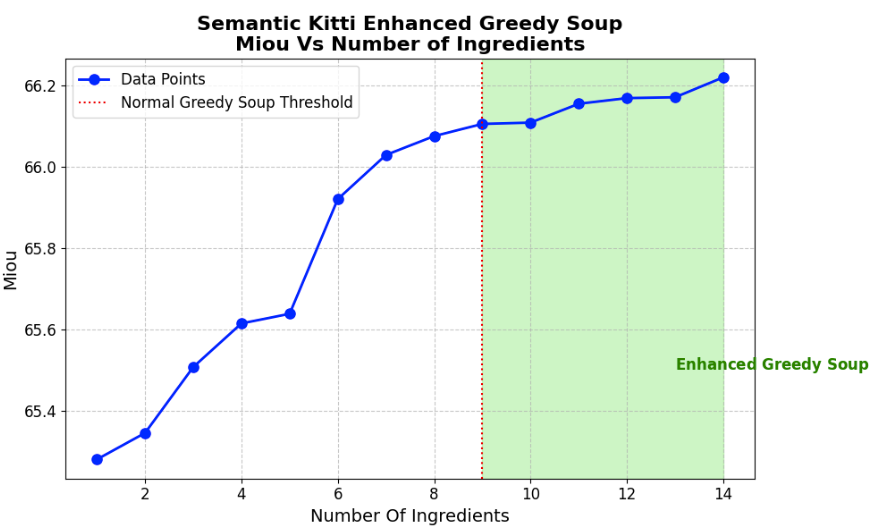
\includegraphics[width=0.5\textwidth]{photos/semanticKitti.png}
    \caption{Enhaced Greedy Soup improves 1\% on best checkpoint }
    \label{fig:photo_example}
\end{figure}

\begin{table}[htbp]
\centering
\small

\begin{tabular}{|l|l|l|}
\hline
\textbf{Ingredients} & \textbf{Count} & \textbf{MIoU (\%)} \\
\hline
$[0]$ & 1 & 75.7099\\
$[0,1]$ & 2 & 75.8291\\
$[0,1,2]$ & 3 & 75.8732 \\
$[0,1,2,3]$ & 4 & 75.9178 \\
$[0,1,2,3,4]$ & 5 & 76.0154 \\
$[0,1,2,3,4,15]$ & 6 & 76.0245 \\
$[0,1,2,3,4,15,21]$ & 7 & 76.0398 \\
$[0,1,2,3,4,15,21,29]$ & 8 & 76.0656 \\
$[0,1,2,3,4,15,21,29,66]$ & 9 & 76.0809 \\
$[0,1,2,3,4,15,21,29,66,73]$ & 10 & 76.0812 \\
$[0(2),1,2,3,4,15,21,29,66,73]$ & 11 & 76.0912 \\
$[0(2),1(2),2,3,4,15,21,29,66,73]$ & 12 & 76.1110 \\
$[0(2),1(2),2,3,4(2),15,21,29,66,73]$ & 13 & 76.1297 \\
$[0(2),1(2),2,3,4(2),15,21(2),29,66,73]$ & 14 & 76.1323 \\
$[0(2),1(2),2,3,4(2),15,21(2),29(2),66,73]$ & 15 & 76.1368 \\
\hline
\end{tabular}
\caption{Nuscenes MIoU values for different ingredient combinations}
\end{table}


\begin{figure}[h]
    \centering
    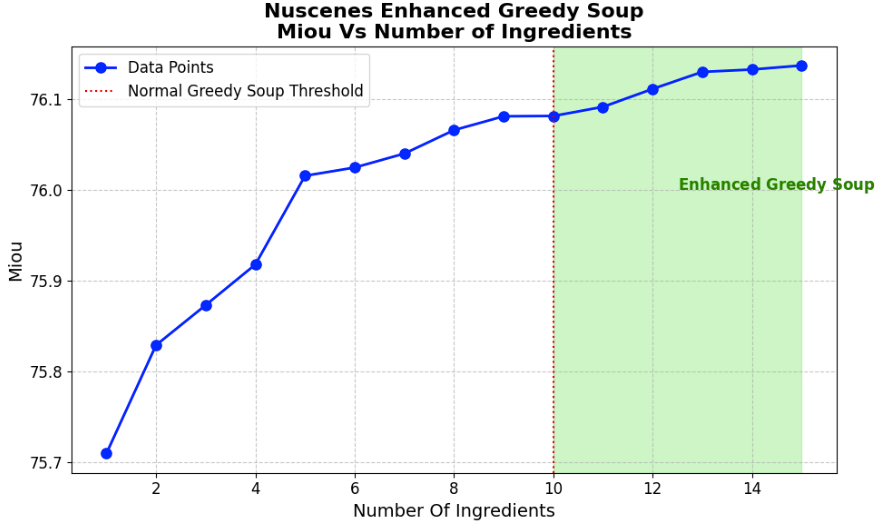
\includegraphics[width=0.5\textwidth]{photos/nuscenes.png}
    \caption{Enhaced Greedy Soup improves 0.5\% on best checkpoint }
    \label{fig:photo_example}
\end{figure}


\section{Conclusion}

We introduce a groundbreaking methodology named "Iterative Scan Greedy Model Soup" that we have applied to the realm of LiDAR semantic segmentation. By harnessing this innovative approach, we enhance an advanced open-source 2DPASS \cite{yan20222dpass} semantic segmentation code and showcase its effectiveness on the semanticKitti and nuscenes datasets. Significantly, our technique achieves remarkable enhancements in Mean Intersection Over Union (MIoU) metrics, all while maintaining the prediction time unchanged.


\section{References}


%%%%%%%%% REFERENCES
\bibliographystyle{plain} % Choose a bibliography style
\bibliography{egbib} % Specify the .bib file name without the extension


\end{document}